\documentclass[]{article}

% Imported Packages
%------------------------------------------------------------------------------
\usepackage{amssymb}
\usepackage{amstext}
\usepackage{amsthm}
\usepackage{amsmath}
\usepackage{enumerate}
%\usepackage{fancyhdr}
\usepackage[margin=1in]{geometry}
\usepackage{graphicx}
%\usepackage{extarrows}
%\usepackage{setspace}
\usepackage{float}
\usepackage[hidelinks]{hyperref}

% Configure Packages
%------------------------------------------------------------------------------
\hypersetup{linktoc=all}
\graphicspath{{Resources/}}
%------------------------------------------------------------------------------

% Header and Footer
%------------------------------------------------------------------------------
\pagestyle{plain}

\begin{document}
\cleardoublepage
\pagenumbering{gobble}
\begin{titlepage}
	\newcommand{\HRule}{\rule{\linewidth}{0.5mm}} % Defines a new command
	%for the
	%horizontal lines, change thickness heReve
	\center % Center everything on the page

	%----------------------------------------------------------------------------------------
	%	HEADING SECTIONS
	%----------------------------------------------------------------------------------------

	\textsc{\LARGE McMaster University}\\[1.5cm] % Name of your
	%university/college
	\textsc{\Large Software Design II \\  \Large Large System Design}\\[0.5cm] % Major heading
	%such as course name
	\textsc{\large SFWR ENG 3A04}\\[0.5cm] % Minor heading such as course
	%title

	%----------------------------------------------------------------------------------------
	%	TITLE SECTION
	%----------------------------------------------------------------------------------------

	\HRule \\[0.4cm]
	{ \huge \bfseries Deliverable \# 2}\\[0.4cm] % Title of your
	%document
	\HRule \\[1.5cm]

	%----------------------------------------------------------------------------------------
	%	AUTHOR SECTION
	%----------------------------------------------------------------------------------------

	\Large \emph{Authors:}\\
	Alexander \textsc{Jackson} \textbf{1302526} \\
	Harit \textsc{Patel} \textbf{1317372} \\ %Add your student number
	Josh \textsc{Voskamp} \textbf{1319352} \\
	Lucas \textsc{Bongers} \textbf{1202472} \\
	Mohammad \textsc{Naveed} \textbf{1332196} \\[3cm]
	%----------------------------------------------------------------------------------------
	%	DATE SECTION
	%----------------------------------------------------------------------------------------

	{\large \today}\\[3cm] % Date, change the \today to a set date if you
	%want to be precise

	\vfill % Fill the rest of the page with whitespace

\end{titlepage}

% Table of Contents
% Start numbering pages after ToC
\tableofcontents
\cleardoublepage
\pagenumbering{arabic}

\section{Introduction}
\label{sec:introduction}
% Begin Section


\subsection{Purpose}
\label{sub:purpose}
% Begin SubSection

The purpose of this document is to provide the developers with the architectural design of the system-to-be. Furthermore, this document also includes diagrams that provide insight on system architecture and structure. The intended audience for this document are the developers, TA's, and Dr. Khedri.

% End SubSection

\subsection{System Description}
\label{sub:system_description}
% Begin SubSection

The application will identify land animals by presenting a series of questions to the user. The application will then produce a list of known animals that best match the answers entered by the user. With each possible match, the application will display basic information about the animal as well as a link to a webpage where the user can find more detailed information. In addition, the application will retain a list of recent animals spotted by the user, including marking on Google Maps the location of the user when each animal was sighted.
\\
\\
The application is designed to run on an Android smart-phone. The application will require the use of the Google Maps API, and will depend on the smart-phone having Internet access and location permissions. The application is designed to be self-contained and will not access any files on the device other than its own.

% End SubSection

\subsection{Overview}
\label{sub:overview}
% Begin SubSection

The rest of this document contains information about the architectural design of the application and its subsytems. Section 2 of this document features a use case diagram of the application, with a text description for each use case, and section 3 contains the corresponding analysis class diagram. Section 4 provides an overview of the overall architectural design of the application. This overview includes justification of the overall architecture, a division of the system into subsystems, and explanation of the relationships between subsystems. Section 6 contains a list of all class responsibility collaboration (CRC) cards, with a CRC card provided for each identified class in the system-to-be. The final section in this document is a division of labour section that indicates the contributions of each individual to this document.

% End SubSection

% End Section

\section{Use Case Diagram}
\label{sec:use_case_diagram}
% Begin Section
%This section should provide a use case diagram for your application.
\begin{figure}[H]
	\centering
	\includegraphics[width = 14cm]{UseCaseDiagram}
	\caption{Use Case Diagram}
	\label{Use Case Diagram}
\end{figure}

\begin{enumerate}[a)]
	\item Help: Lets the user view FAQ's, bug fixes, and change log.

	\item Settings: Section for the user to change app settings: view help menu, view/delete sighting history, select used experts. Extends help section, sighting history, and selecting available experts.

	\item Identify Animal: Starts the animal identification process, includes consult experts and uses location. The results will be displayed to the central forum after the experts have made their decisions.

	\item Consult Experts: A stage in the process of identifying an animal, relies on animal and geographic consultants to ensure accuracy. The experts present a series of questions to the user and decide on possible matches based on the answers.

	\item Sighting History: Contains the most recent animals sighted by the user, and basic information about the animal, and when and where it was sighted. User can delete specific entries or the whole list.

	\item Select Available Experts: Lets the user select which experts to activate/deactivate for use in identifying animals. The user must have at least one expert selected, and cannot choose more than 5 to be in use at a time.

	\item Add Experts: When the development team adds a new expert for users to select for animal identification. The user will be able to select the new expert in the select available experts section.

	\item Remove Experts: When the development team removes an existing expert from the system. The removed expert will no longer be available for selection in the select available experts section, and users who currently have it selected for use will be prompted to select a different expert.

	\item location: The app gets the user's location at the beginning of each animal identification process, and logs it with the animal sighting history.

	\item Encrypt Data: The security consultant must ensure user data and information communicated by the experts is secure
\end{enumerate}
% End Section

\section{Analysis Class Diagram}
\label{sec:analysis_class_diagram}
% Begin Section
% This section should provide an analysis class diagram for your application.
\begin{figure}[H]
	\centering
	\includegraphics[width = 14cm]{ACDV2}
	\caption{Analysis Class Diagram}
	\label{Analysis Class Diagram}
\end{figure}
% End Section


\section{Architectural Design}
\label{sec:architectural_design}
% Begin Section
% This section should provide an overview of the overall architectural design of your application. You overall architecture should show the division of the system into subsystems with high cohesion and low coupling.

\subsection{System Architecture}
\label{sub:system_architecture}
% Begin SubSection
\begin{enumerate}[a)]
	\item The system will be designed using the blackboard version of a data centered architecture.
	\item The agents or knowledge stores of the data store are the experts of the system which will be working independently of each other, they will only interact with the blackboard. When the animal identification process is started the data store will call on the experts to start a decision making process based on the answers the user provides to the questions asked by the experts. The experts will post their decisions to the central forum for the user to view after the process has been completed. The blackboard will contain the knowledge entered by the user, and the experts will contain the rules used to sort the knowledge contained in the blackboard.
	\item The system will use the blackboard style architecture because the app is based on a decision making process. The experts may not always agree on the result since they are all contributing and drawing from different areas of knowledge, and so they will all contribute different views. The most likely of these views are the ones that will be posted to the central forum for the user to view.
\end{enumerate}
\begin{figure}[H]
	\centering
	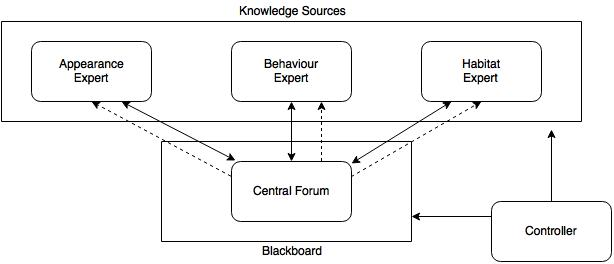
\includegraphics[width = 14cm]{Subsystem_Architecture}
	\caption{Subsystem Architecture}
	\label{Subsystem Architecture}
\end{figure}
% End SubSection

\subsection{Subsystems}
\label{sub:subsystems}
% Begin SubSection
\begin{enumerate}[a)]
	\item Blackboard Subsystem: The purpose of this system is to store all the knowledge and to call on the experts to reach decisions based on the knowledge in the central forum. It prompts the knowledge source subsystem and is controlled by the controller subsystem.
	\item Knowledge Subsystem: The purpose of this system is to make decisions on the data contained in the data store when prompted by the blackboard. The classes in the knowledge source subsystem communicate only with the blackboard and not with each other. This subsystem is prompted by the blackboard subsystem and controlled by the controller subsystem.
	\item Controller Subsystem: The responsibility of this system is to have overall supervision of the entire system and to initiate the knowledge and blackboard subsystems.
\end{enumerate}
% End SubSection

% End Section

\section{Class Responsibility Collaboration (CRC) Cards}
\label{sec:class_responsibility_collaboration_crc_cards}
% Begin Section
%This section should contain all of your CRC cards.

% \begin{enumerate}[a)]
% 	\item Provide a CRC Card for each identified class
% 	\item Please use the format outlined in tutorial, i.e.,
% 	\begin{table}[ht]
% 		\centering
% 		\begin{tabular}{|p{5cm}|p{5cm}|}
% 		\hline
% 		 \multicolumn{2}{|l|}{\textbf{Class Name:}} \\
% 		\hline
% 		\textbf{Responsibility:} & \textbf{Collaborators:} \\
% 		\hline
% 		\vspace{1in} & \\
% 		\hline
% 		\end{tabular}
% 	\end{table}
%
% \end{enumerate}
\begin{table}[H]
	\centering
	\begin{tabular}{|p{5cm}|p{5cm}|}
		\hline
		\multicolumn{2}{|l|}{\textbf{IdentificationControl}} \\
		\hline
		\textbf{Responsibility:} & \textbf{Collaborators:} \\
		\hline
		 Controller class that calls collaborators to identify an animal and passes results to GUIControl to display results and store result in sighting history & BehaviourExpertControl \break AppearanceExpertControl \break HabitatExpertControl \break GUIControl\\
		\hline
	\end{tabular}
\end{table}
\begin{table}[H]
	\centering
	\begin{tabular}{|p{5cm}|p{5cm}|}
		\hline
		\multicolumn{2}{|l|}{\textbf{BehaviourExpertControl}} \\
		\hline
		\textbf{Responsibility:} & \textbf{Collaborators:} \\
		\hline
		 Controller class that controls interactions and requests for the Behaviour Expert & BehaviourExpertEntity \break IdentificationControl\\
		\hline
	\end{tabular}
\end{table}
\begin{table}[H]
	\centering
	\begin{tabular}{|p{5cm}|p{5cm}|}
		\hline
		\multicolumn{2}{|l|}{\textbf{AppearanceExpertControl}} \\
		\hline
		\textbf{Responsibility:} & \textbf{Collaborators:} \\
		\hline
		 Controller class that controls interactions and requests for the Appearance Expert & AppearanceExpertEntity \break IdentificationControl\\
\hline
	\end{tabular}
\end{table}
\begin{table}[H]
	\centering
	\begin{tabular}{|p{5cm}|p{5cm}|}
		\hline
		\multicolumn{2}{|l|}{\textbf{HabitatExpertControl}} \\
		\hline
		\textbf{Responsibility:} & \textbf{Collaborators:} \\
		\hline
		 Controller class that controls interactions and requests for the Habitat Expert & HabitatExpertEntity \break IdentificationControl\\
\hline
	\end{tabular}
\end{table}
\begin{table}[H]
	\centering
	\begin{tabular}{|p{5cm}|p{5cm}|}
		\hline

		\multicolumn{2}{|l|}{\textbf{BehaviourExpertEntity}} \\
		\hline
		\multicolumn{2}{|l|}{\textbf{SightingHistroy}} \\\hline
		\textbf{Responsibility:} & \textbf{Collaborators:} \\
		\hline
		 Entity class that contains information necessary to identify animal based on its behaviour & BehaviourExpertControl\\
\hline
	\end{tabular}
\end{table}
\begin{table}[H]
	\centering
	\begin{tabular}{|p{5cm}|p{5cm}|}
		\hline
		\multicolumn{2}{|l|}{\textbf{AppearanceExpertEntity}} \\
		\hline
		\textbf{Responsibility:} & \textbf{Collaborators:} \\
		\hline
		 Entity class that contains information necessary to identify animal based on its appearance & AppearanceExpertControl\\
		\hline

	\end{tabular}
\end{table}
\begin{table}[H]
	\centering
	\begin{tabular}{|p{5cm}|p{5cm}|}
		\hline
		\multicolumn{2}{|l|}{\textbf{HabitatExpertEntity}} \\
		\hline
		\textbf{Responsibility:} & \textbf{Collaborators:} \\
		\hline
		 Entity class that contains information necessary to identify animal based on its habitat & HabitatExpertControl\\
\hline
	\end{tabular}
\end{table}
\begin{table}[H]
	\centering
	\begin{tabular}{|p{5cm}|p{5cm}|}
		\hline
		\multicolumn{2}{|l|}{\textbf{GUIControl}} \\
		\hline
		\textbf{Responsibility:} & \textbf{Collaborators:} \\
		\hline
		 Controller class that interfaces  between the animal identification process and the UI classes and home screen & IdentificationControl \break Results \break SightingHistory \break SelectExperts \break AnswerQuestion \break Help \break IdentifyAnimal \break Settings\\
\hline
	\end{tabular}
\end{table}
\begin{table}[H]
	\centering
	\begin{tabular}{|p{5cm}|p{5cm}|}
		\hline
		\multicolumn{2}{|l|}{\textbf{Results}} \\
		\hline
		\textbf{Responsibility:} & \textbf{Collaborators:} \\
		\hline
		Show results of animal identification process and allow user to select correctly identified animal from list & GUIControl\\
		\hline

	\end{tabular}
\end{table}
\begin{table}[H]
	\centering
	\begin{tabular}{|p{5cm}|p{5cm}|}
		\hline
		\multicolumn{2}{|l|}{\textbf{SightingHistory}} \\
		\hline
		\textbf{Responsibility:} & \textbf{Collaborators:} \\
		\hline
		 Allows user to view and delete animal sighting history & GUIControl \\
\hline
	\end{tabular}
\end{table}
\begin{table}[H]
	\centering
	\begin{tabular}{|p{5cm}|p{5cm}|}
		\hline
		\multicolumn{2}{|l|}{\textbf{SelectExperts}} \\
		\hline
		\textbf{Responsibility:} & \textbf{Collaborators:} \\
		\hline
		 Lets user select which experts will be called on during future animal identification processes & GUIControl \\
\hline
	\end{tabular}
\end{table}
\begin{table}[H]
	\centering
	\begin{tabular}{|p{5cm}|p{5cm}|}
		\hline
		\multicolumn{2}{|l|}{\textbf{AnswerQuestion}} \\
		\hline
		\textbf{Responsibility:} & \textbf{Collaborators:} \\
		\hline
		 Allows user to answer question presented by experts during the animal identification process & GUIControl \\
\hline
	\end{tabular}
\end{table}
\begin{table}[H]
	\centering
	\begin{tabular}{|p{5cm}|p{5cm}|}
		\hline
		\multicolumn{2}{|l|}{\textbf{Help}} \\
		\hline
		\textbf{Responsibility:} & \textbf{Collaborators:} \\
		\hline
		 Boundary class that displays help information such as FAQs, how to use the app and troubleshooting & GUIControl\\
		\hline
	\end{tabular}
\end{table}
\begin{table}[H]
	\centering
	\begin{tabular}{|p{5cm}|p{5cm}|}
		\hline
		\multicolumn{2}{|l|}{\textbf{IdentifyAnimal}} \\
		\hline
		\textbf{Responsibility:} & \textbf{Collaborators:} \\
		\hline
		 Allows user to begin the animal identification process & GUIControl \\
\hline
	\end{tabular}
\end{table}

% End Section

\newpage
\section*{Division of Labour}
\label{sec:division_of_labour}
\addcontentsline{toc}{section}{Division of Labour}
% Begin Section
%Include a Division of Labour sheet which indicates the contributions of each team member. This sheet must be signed by all team members.
\begin{table}[H]
	\centering
	\begin{tabular}{|p{5cm}|p{2cm}|p{3.5cm}|p{3cm}|}\hline
	    \textbf{Revisions Made} & \textbf{Date} & \textbf{Reason for Revision} & \textbf{Revising Party}\\\hline
		Added title page & 2016/02/11 & Document Creation & Josh Voskamp\\\hline
		Added introduction & 2016/03/03 & Document Addition & Alexander Jackson\\\hline
		Added use case descriptions, system architecture and diagram, and subsystem breakdown & 2016/03/05 & Document Addition & Lucas Bongers\\\hline
		Added Use Case Diagram, Analysis Class Diagram, CRC Cards & 2016/03/05 & Document Addition & Josh Voskamp, \break Mohammad Naveed, \break Harit Patel\\\hline
		Added new version of analysis class diagram & 2016/03/17 & Document Addition & Lucas Bongers\\\hline
		Changed all CRC cards based on new analysis class diagram & 2016/03/17 & Document Addition & Lucas Bongers\\\hline
	\end{tabular}
\end{table}
\vspace{3cm}
\section*{Signatures}
\vspace{1cm}
\noindent Alexander Jackson \\\hrule
\vspace{1cm}
\noindent Harit Patel \\\hrule
\vspace{1cm}
\noindent Josh Voskamp \\\hrule
\vspace{1cm}
\noindent Lucas Bongers \\\hrule
\vspace{1cm}
\noindent Mohammad Naveed \\\hrule
% \section*{IMPORTANT NOTES}
% \begin{itemize}
% %	\item You do \underline{NOT} need to provide a text explanation of each diagram; the diagram should speak for itself
% 	\item Please document any non-standard notations that you may have used
% 	\begin{itemize}
% 		\item \emph{Rule of Thumb}: if you feel there is any doubt surrounding the meaning of your notations, document them
% 	\end{itemize}
% 	\item Some diagrams may be difficult to fit into one page
% 	\begin{itemize}
% 		\item It is OK if the text is small but please ensure that it is readable when printed
% 		\item If you need to break a diagram onto multiple pages, please adopt a system of doing so and thoroughly explain how it can be reconnected from one page to the next; if you are unsure about this, please ask about it
% 	\end{itemize}
% 	\item Please submit the latest version of Deliverable 1 with Deliverable 2
% 	\begin{itemize}
% 		\item It does not have to be a freshly printed version; the latest marked version is OK
% 	\end{itemize}
% 	\item If you do \underline{NOT} have a Division of Labour sheet, your deliverable will \underline{NOT} be marked
% \end{itemize}
%

\end{document}
%------------------------------------------------------------------------------
